\documentclass[12pt, twoside]{article}
% \documentclass[12pt, twoside]{article}
\usepackage[letterpaper, margin=1in, headsep=0.2in]{geometry}
\setlength{\headheight}{0.6in}
%\usepackage[english]{babel}
\usepackage[utf8]{inputenc}
\usepackage{microtype}
\usepackage{amsmath}
\usepackage{amssymb}
%\usepackage{amsfonts}
\usepackage[nomessages]{fp} %\FPeval{\var-name}{2*sin(pi/6)}
\usepackage{siunitx} %units in math. eg 20\milli\meter
\usepackage{yhmath} % for arcs, overparenth command
\usepackage{tikz} %graphics
\usetikzlibrary{quotes, angles, arrows, arrows.meta}
\usepackage{graphicx} %consider setting \graphicspath{{images/}}
\usepackage{parskip} %no paragraph indent
\usepackage{enumitem}
\usepackage{multicol}
\usepackage{venndiagram}

\usepackage{fancyhdr}
\pagestyle{fancy}
\fancyhf{}
\renewcommand{\headrulewidth}{0pt} % disable the underline of the header
\raggedbottom
\hfuzz=2mm %suppresses overfull box warnings

\usepackage{hyperref}
\usepackage{float}

\title{Algebra 2}
\author{Chris Huson}
\date{September 2024}

\fancyhead[RO]{\\ First and last name: \hspace{2.5cm} \,\\ Section: \hspace{2.5cm} \,}
\fancyhead[LO]{BECA/Huson/Geometry: Construction \\* 25 September 2024}

\begin{document}
\subsubsection*{1.15 Do Now: Transformations and constructions}
\begin{enumerate}[itemsep=0.5cm]


\item Reflect $\triangle ABC$ across the $y$-axis. Label the image $\triangle A'B'C'$.
\begin{center}
    \begin{tikzpicture}[scale=.48]
    \draw [help lines] (-7,-4) grid (7,6);
    \draw [thick, <->] (-7.4,0) -- (7.4,0) node [right] {$x$};
    \draw [thick, <->] (0,-4.4)--(0,6.4) node [above] {$y$};  
    \draw [thick]
      (-2,-2) node[below] {$A$}--
      (-5,4) node[left] {$B$}--
      (-5,-2) node[below] {$C$}--cycle;  
\end{tikzpicture}
\end{center}

\item Rotate $\triangle ABC$ $90^\circ$ counterclockwise around the origin. Label the image $\triangle A'B'C'$.
  \begin{center}
      \begin{tikzpicture}[scale=.48]
      \draw [help lines] (-6,-4) grid (6,7);
      \draw [thick, <->] (-6.4,0) -- (6.4,0) node [right] {$x$};
      \draw [thick, <->] (0,-4.4)--(0,7.4) node [above] {$y$};  
      \draw [thick]
        (0,0) node[below left] {$A$}--
        (3,5) node[right] {$B$}--
        (3,0) node[below right] {$C$}--cycle;  
    \end{tikzpicture}
  \end{center}
  

\item Use the function $f(x) = 8x+3$ to answer the questions.
  \begin{multicols}{2}
  \begin{enumerate}[itemsep=2cm]
      \item What is $f(0)$?
      \item Find $f(\frac{1}{4})$
      \item Solve for $x$ if $f(x) = -13$.
  \end{enumerate}
  \end{multicols} \vspace{1cm}

\newpage
\subsubsection*{Constructions: Use only a compass and straightedge}

\item Construct an equilateral triangle with one side $\overline{AB}$.  [Leave all construction marks.]
\vspace{2cm}
\begin{center}
\begin{tikzpicture}
  \draw [-, thick] (0,0)--(0,5);
  \draw [fill] (0,0) circle [radius=0.05] node[right]{$A$};
  \draw [fill] (0,5) circle [radius=0.05] node[right]{$B$};
\end{tikzpicture}
\end{center} \vspace{1cm}


\item Construct an angle bisector the given angle $A$.  [Leave all construction marks.]
  \vspace{2cm}
  \begin{center}
  \begin{tikzpicture}
    \draw [<->, thick] (3,6)--(0,0)--(8,0);
    \draw [fill] (0,0) circle [radius=0.05] node[below]{$A$};
    %\draw [fill] (7,0) circle [radius=0.05] node[below]{$N$};
  \end{tikzpicture}
  \end{center}

\newpage
\item Construct a perpendicular bisector of side $\overline{AC}$ of the triangle. Label the midpoint of $\overline{AC}$ as $M$. Connect the points $M$ and $B$ with a line, a median of the triangle.  
    \vspace{5cm}
    \begin{center}
    \begin{tikzpicture}
        \draw [-, thick] (0,0)--(10,0)--(8,5)--cycle;
        \draw [fill] (0,0) circle [radius=0.05] node[above left]{$A$};
        %\node at (8.5,-0.4){$l$};
        \draw [fill] (10,0) circle [radius=0.05] node[below right]{$B$};
        \draw [fill] (8,5) circle [radius=0.05] node[above right]{$C$};

    \end{tikzpicture}
    \end{center}
    \vspace{2cm}




\end{enumerate}
\end{document}